\subsection{Módulo de radio}
El modelo de radio elegido ha sido el Sintonizador FM RDA5807M, mostrado en la \autoref{fig:2-3-Radio},  utilizado anteriormente en la asignatura de Sistemas Basados en Microprocesadores.

Dicho modelo se comunica con el microcontrolador mediante el protocolo \texttt{I2C}. El sintonizador cuenta con un decodificador MPX, salida de audio stereo y un rango de sintonización de 87 MHz a 108 MHz debido a nuestra situación geográfica.

En cuanto a la señal de audio de salida, hemos encontrado que presenta una componente continua de 1.65V y el mismo valor de amplitud, es decir, una señal de 3.3V pico a pico centrada en 1.65V.

Todas las características de dicho sintonizador FM se han obtenido del datasheet ofrecido por el fabricante.

\begin{figure}[h]
    \centering
    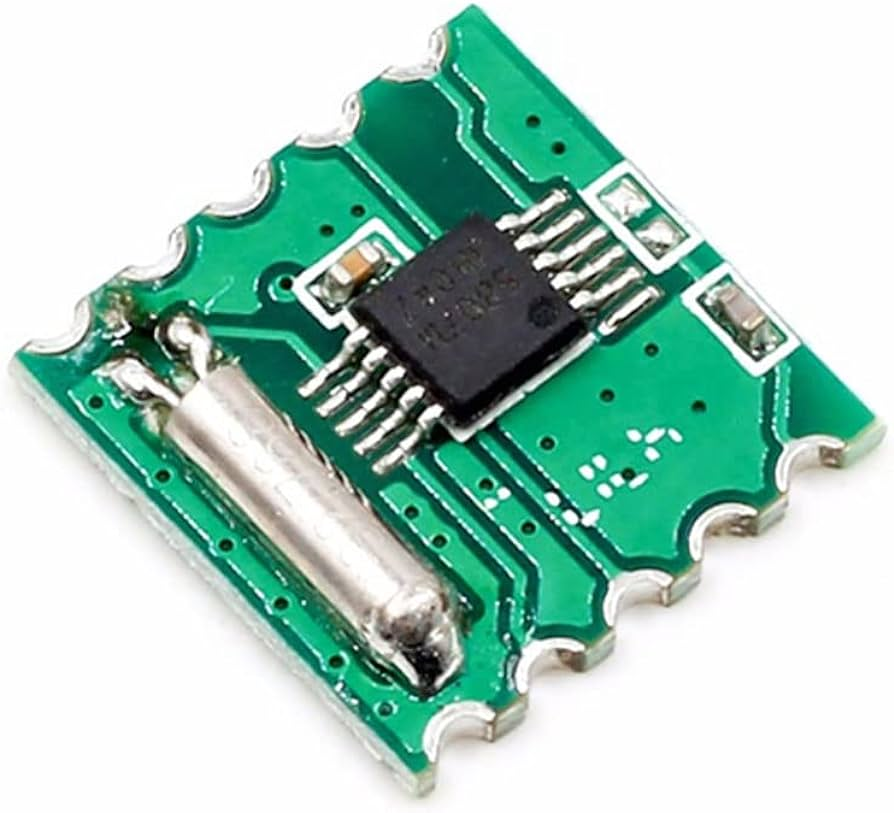
\includegraphics[width=0.3\textwidth]{images/2/2-3/Radio.jpg}
    \caption{Sintonizador FM RDA5807M}
    \label{fig:2-3-Radio}
\end{figure}